\section{Experimento BRDF Cook-Torrance Alternativa}

Este experimento é uma versão alternativa da feita na \autoref{sec:cook-torrance}. As equações na \autoref{fig-cook-torrance-alternative-eqlang-latex} fazem uso da equação do Efeito Fresnel e foram escolhidas constantes diferentes. Código fonte em \texttt{EquationLang} pode ser visto no \autoref{cod-cook-torrance-alternative-eqlang}. Os códigos gerados em GLSL estão no \autoref{cod-cook-torrance-alternative-glsl-pt-1} e \autoref{cod-cook-torrance-alternative-glsl-pt-2}. Objetos 3D renderizados pode ser vistos na \autoref{fig-cook-torrance-alternative-eqlang} e os plots estão na \autoref{fig-cook-torrance-alternative-plots}.

%%%%%%%%%%%%%%%%%%%%%%%%%%%%%%%%%%%%%%%%%%%%%%%%%
\subsection{Representação em documento \LaTeX{}}
%%%%%%%%%%%%%%%%%%%%%%%%%%%%%%%%%%%%%%%%%%%%%%%%%
\begin{figure}[H]
    \caption{\label{fig-cook-torrance-alternative-eqlang-latex} \small Equações da BRDF do experimento cook-torrance-alternative em documento \LaTeX{}.}
    \begin{center}
        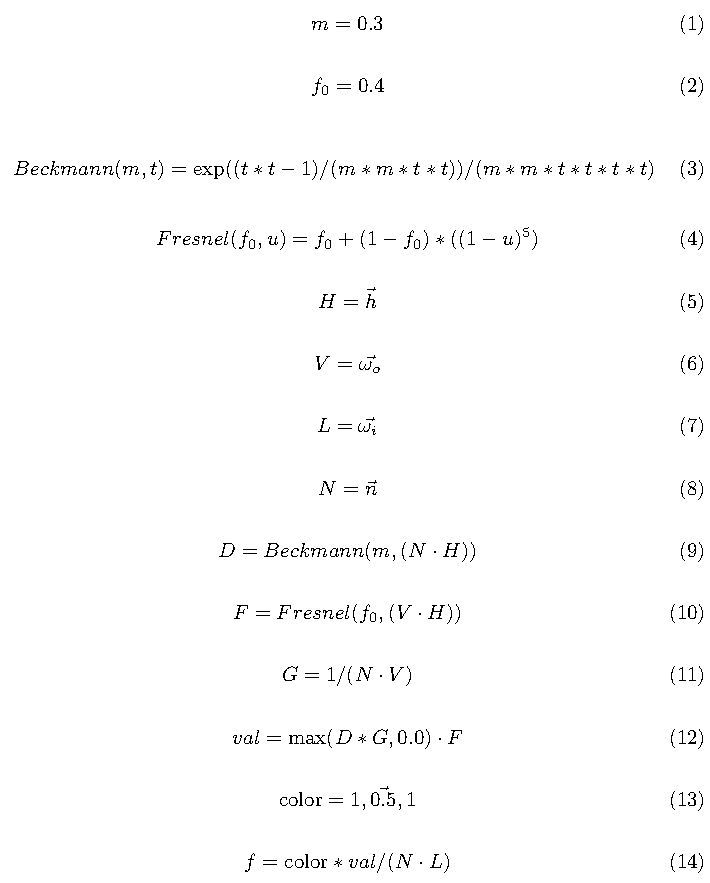
\includegraphics[scale=0.92]{./Imagens/brdfs/cook-torrance-alternative.pdf}
    \end{center}
\end{figure}

%%%%%%%%%%%%%%%%%%%%%%%%%%%%%%%%%%%%%%%%%%%%%%%%%
\subsection{Visualização do Resultado}
%%%%%%%%%%%%%%%%%%%%%%%%%%%%%%%%%%%%%%%%%%%%%%%%%
\begin{figure}[H]
    \caption{\small{\textit{Plots} da BRDF deste experimento.}}\label{fig-cook-torrance-alternative-plots}
\minipage{0.48\textwidth}
    \vspace{42px}
  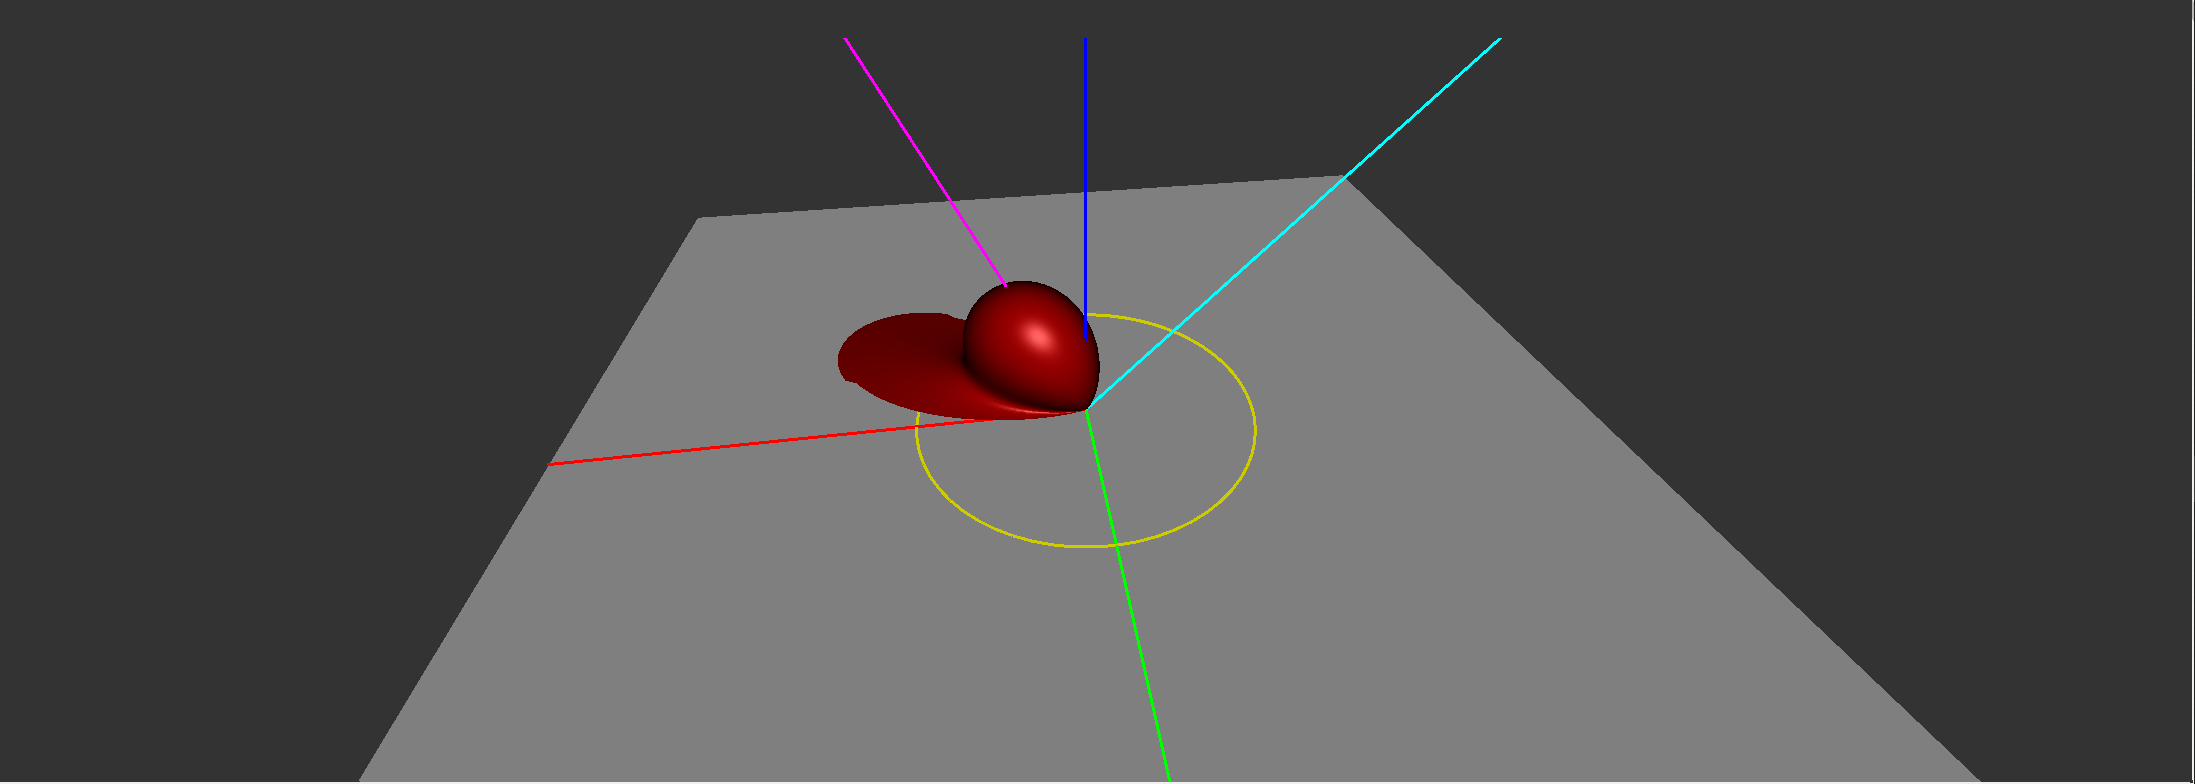
\includegraphics[width=\linewidth]{./Imagens/brdfs/cook-torrance-alternative-3D-plot}
    % \vspace{0.1px}
    \legend{ \small (a) 3D \textit{plot}}
\endminipage\hfill
\minipage{0.48\textwidth}
  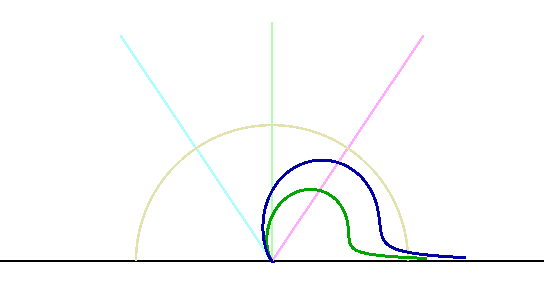
\includegraphics[width=\linewidth]{./Imagens/brdfs/cook-torrance-alternative-polar-plot-log.png}
    \legend{ \small (b) \textit{Polar plot}}
\endminipage\hfill
\end{figure}

\begin{figure}[H]
    \caption{\small{Objetos 3D renderizados por este experimento}}\label{fig-cook-torrance-alternative-eqlang}
\minipage{0.32\textwidth}
  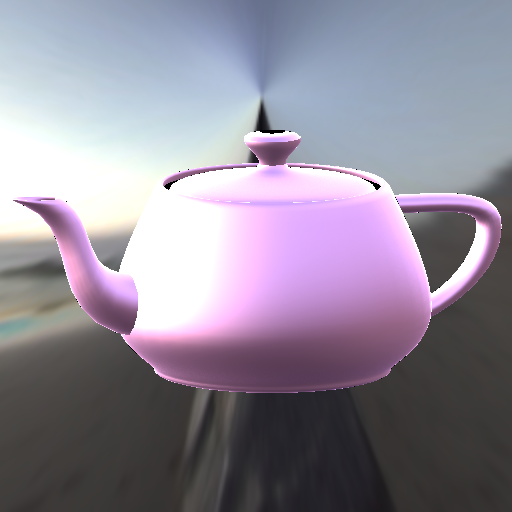
\includegraphics[width=\linewidth]{./Imagens/brdfs/cook-torrance-alternative-teapot.png}
    \legend{ \small (a) \textit{Teapot}}
\endminipage\hfill
\minipage{0.32\textwidth}
  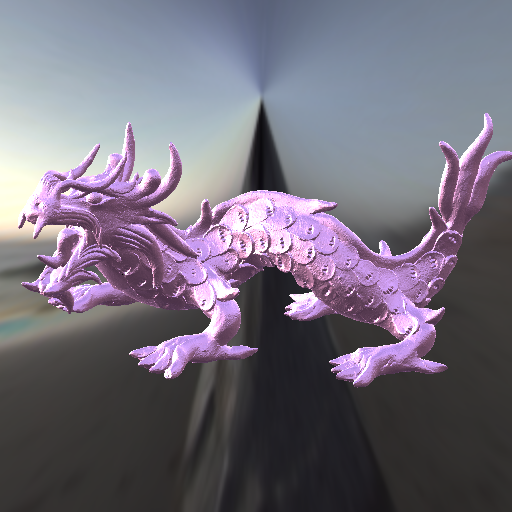
\includegraphics[width=\linewidth]{./Imagens/brdfs/cook-torrance-alternative-dragon.png}
    \legend{ \small (b) Dragão de Stanford}
\endminipage\hfill
\minipage{0.32\textwidth}%
  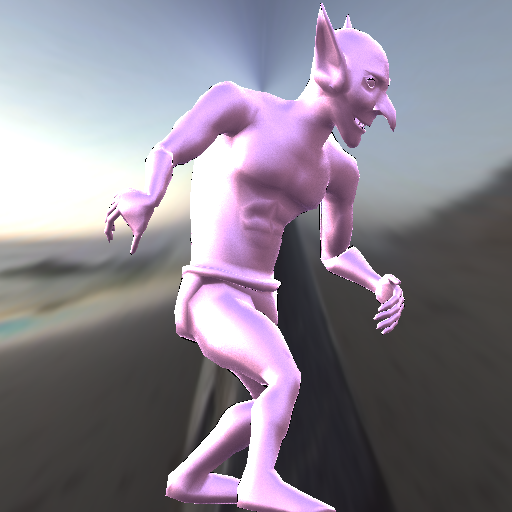
\includegraphics[width=\linewidth]{./Imagens/brdfs/cook-torrance-alternative-goblin.png}
    \legend{ \small (c) Goblin}
\endminipage
\end{figure}

%%%%%%%%%%%%%%%%%%%%%%%%%%%%%%%%%%%%%%%%%%%%%%%%%
\subsection{Código GLSL Gerado}
%%%%%%%%%%%%%%%%%%%%%%%%%%%%%%%%%%%%%%%%%%%%%%%%%
\begin{codigo}[H]
    \caption{\small Saida do compilador, código GLSL da BRDF deste experimento (parte 1). }
    \label{cod-cook-torrance-alternative-glsl-pt-1}
\begin{lstlisting}[language=C, inputencoding=utf8]
analytic ::begin parameters
#[type][name][min val][max val][default val]
::end parameters
::begin shader
//////////// START OF BUILTINS DECLARTION ////////////
vec3 var_0_vec_h;
vec3 var_3_vec_n;
float var_10_theta_h;
float var_11_theta_d;
float var_1_pi;
float var_2_epsilon;
vec3 var_4_vec_omega_i;
float var_5_theta_i;
float var_6_phi_i;
vec3 var_7_vec_omega_o;
float var_8_theta_o;
float var_9_phi_o;
//////////// END OF BUILTINS DECLARTION ////////////
//////////// START OF USER DECLARED ////////////
vec3 var_12_V;
vec3 var_13_L;
float var_17_f_0;
float var_15_m;
vec3 var_20_H;
vec3 var_21_text_color;
vec3 var_22_N;
float var_23_D;
float var_24_G;
float var_25_F;
float var_26_val;
vec3 var_27_f;
\end{lstlisting}
\end{codigo}

\begin{codigo}[H]
    \caption{\small Saida do compilador, código GLSL da BRDF deste experimento  (parte 2). }
    \label{cod-cook-torrance-alternative-glsl-pt-2}
\begin{lstlisting}[language=C, inputencoding=utf8]
//////////// END OF USER DECLARED ////////////
//////////// START FUNCTIONS DECLARATIONS ////////////
float var_14_Beckmann(float var_15_m, float var_16_t) {
  return (exp((((((var_16_t * var_16_t) - 1.0)) /
                ((((var_15_m * var_15_m) * var_16_t) * var_16_t))))) /
          ((((((var_15_m * var_15_m) * var_16_t) * var_16_t) * var_16_t) *
            var_16_t)));
}
float var_18_Fresnel(float var_17_f_0, float var_19_u) {
  return (var_17_f_0 + (((1.0 - var_17_f_0)) * (pow(((1.0 - var_19_u)), 5.0))));
}
//////////// END FUNCTIONS DECLARATIONS ////////////
//////////// END FUNCTIONS DECLARATIONS ////////////
vec3 BRDF(vec3 L, vec3 V, vec3 N, vec3 X, vec3 Y) {
  //////////// START OF BUILTINS INITIALIZATION ////////////
  var_0_vec_h = normalize(L + V);
  var_3_vec_n = normalize(N);
  var_1_pi = 3.141592653589793;
  var_2_epsilon = 1.192092896e-07;
  var_4_vec_omega_i = L;
  var_5_theta_i = atan(var_4_vec_omega_i.y, var_4_vec_omega_i.x);
  var_6_phi_i = atan(sqrt(var_4_vec_omega_i.y * var_4_vec_omega_i.y +
                          var_4_vec_omega_i.x * var_4_vec_omega_i.x),
                     var_4_vec_omega_i.z);
  var_7_vec_omega_o = V;
  var_8_theta_o = atan(var_7_vec_omega_o.y, var_7_vec_omega_o.x);
  var_9_phi_o = atan(sqrt(var_7_vec_omega_o.y * var_7_vec_omega_o.y +
                          var_7_vec_omega_o.x * var_7_vec_omega_o.x),
                     var_7_vec_omega_o.z);
  var_10_theta_h = acos(dot(var_0_vec_h, N));
  var_11_theta_d = acos(dot(var_0_vec_h, var_4_vec_omega_i));
  //////////// END OF BUILTINS INITIALIZATION ////////////

  var_12_V = var_7_vec_omega_o;
  var_13_L = var_4_vec_omega_i;
  var_17_f_0 = 0.4;
  var_15_m = 0.3;
  var_20_H = var_0_vec_h;
  var_21_text_color = vec3(1.0, 0.5, 1.0);
  var_22_N = var_3_vec_n;
  var_23_D = var_14_Beckmann(var_15_m, (dot(var_22_N, var_20_H)));
  var_24_G = (1.0 / (dot(var_22_N, var_12_V)));
  var_25_F = var_18_Fresnel(var_17_f_0, (dot(var_12_V, var_20_H)));
  var_26_val = (max((var_23_D * var_24_G), 0.0) * var_25_F);
  var_27_f = ((var_21_text_color * var_26_val) / (dot(var_22_N, var_13_L)));

  return vec3(var_27_f);
}
\end{lstlisting}
\end{codigo}

%%%%%%%%%%%%%%%%%%%%%%%%%%%%%%%%%%%%%%%%%%%%%%%%%
\subsection{Código Fonte em \texttt{EquationLang}}
%%%%%%%%%%%%%%%%%%%%%%%%%%%%%%%%%%%%%%%%%%%%%%%%%
\begin{codigo}[H]
    \caption{\small Código fonte da BRDF deste experimento.}
    \label{cod-cook-torrance-alternative-eqlang}
\begin{lstlisting}[language=tex, frame=none, inputencoding=utf8]
\begin{equation}
    m = 0.3
\end{equation}
\begin{equation}
    f_0 = 0.4
\end{equation}
\begin{equation}
Beckmann(m, t) = \exp((t*t-1)/(m*m*t*t)) / (m*m*t*t*t*t)
\end{equation}
\begin{equation}
    Fresnel(f_0, u) = f_0 + (1 - f_0) * ((1-u)^ 5)
\end{equation}
\begin{equation}
    H = \vec{h}
\end{equation}
\begin{equation}
    V = \vec{\omega_o}
\end{equation}
\begin{equation}
    L = \vec{\omega_{i}}
\end{equation}
\begin{equation}
    N = \vec{n}
\end{equation}
\begin{equation}
    D = Beckmann(m,  (N \cdot H) )
\end{equation}
\begin{equation}
    F = Fresnel(f_0,  (V \cdot H) )
\end{equation}
\begin{equation}
G = 1/(N \cdot V)
\end{equation}
\begin{equation}
    val = \max(D * G, 0.0) \cdot F
\end{equation}
\begin{equation}
    \text{color} = \vec{1,0.5,1}
\end{equation}
\begin{equation}
    f = \text{color} * val / (N \cdot L)
\end{equation}
\end{lstlisting}
\end{codigo}
